%Version 2.1 April 2023
% See section 11 of the User Manual for version history
%
%%%%%%%%%%%%%%%%%%%%%%%%%%%%%%%%%%%%%%%%%%%%%%%%%%%%%%%%%%%%%%%%%%%%%%
%%                                                                 %%
%% Please do not use \input{...} to include other tex files.       %%
%% Submit your LaTeX manuscript as one .tex document.              %%
%%                                                                 %%
%% All additional figures and files should be attached             %%
%% separately and not embedded in the \TeX\ document itself.       %%
%%                                                                 %%
%%%%%%%%%%%%%%%%%%%%%%%%%%%%%%%%%%%%%%%%%%%%%%%%%%%%%%%%%%%%%%%%%%%%%

\documentclass[sn-basic,pdflatex]{sn-jnl}

%%%% Standard Packages
%%<additional latex packages if required can be included here>

\usepackage{graphicx}%
\usepackage{multirow}%
\usepackage{amsmath,amssymb,amsfonts}%
\usepackage{amsthm}%
\usepackage{mathrsfs}%
\usepackage[title]{appendix}%
\usepackage{xcolor}%
\usepackage{textcomp}%
\usepackage{manyfoot}%
\usepackage{booktabs}%
\usepackage{algorithm}%
\usepackage{algorithmicx}%
\usepackage{algpseudocode}%
\usepackage{listings}%
%%%%

%%%%%=============================================================================%%%%
%%%%  Remarks: This template is provided to aid authors with the preparation
%%%%  of original research articles intended for submission to journals published
%%%%  by Springer Nature. The guidance has been prepared in partnership with
%%%%  production teams to conform to Springer Nature technical requirements.
%%%%  Editorial and presentation requirements differ among journal portfolios and
%%%%  research disciplines. You may find sections in this template are irrelevant
%%%%  to your work and are empowered to omit any such section if allowed by the
%%%%  journal you intend to submit to. The submission guidelines and policies
%%%%  of the journal take precedence. A detailed User Manual is available in the
%%%%  template package for technical guidance.
%%%%%=============================================================================%%%%

\setcounter{secnumdepth}{0}


\raggedbottom




% tightlist command for lists without linebreak
\providecommand{\tightlist}{%
  \setlength{\itemsep}{0pt}\setlength{\parskip}{0pt}}

% From pandoc table feature
\usepackage{longtable,booktabs,array}
\usepackage{calc} % for calculating minipage widths
% Correct order of tables after \paragraph or \subparagraph
\usepackage{etoolbox}
\makeatletter
\patchcmd\longtable{\par}{\if@noskipsec\mbox{}\fi\par}{}{}
\makeatother
% Allow footnotes in longtable head/foot
\IfFileExists{footnotehyper.sty}{\usepackage{footnotehyper}}{\usepackage{footnote}}
\makesavenoteenv{longtable}




\begin{document}


\title[]{Predicting Language Outcomes for 12-month-old Infants From
Low-Income Families: A Machine Learning Approach based on Demographics
Data at Birth}

%%=============================================================%%
%% Prefix	-> \pfx{Dr}
%% GivenName	-> \fnm{Joergen W.}
%% Particle	-> \spfx{van der} -> surname prefix
%% FamilyName	-> \sur{Ploeg}
%% Suffix	-> \sfx{IV}
%% NatureName	-> \tanm{Poet Laureate} -> Title after name
%% Degrees	-> \dgr{MSc, PhD}
%% \author*[1,2]{\pfx{Dr} \fnm{Joergen W.} \spfx{van der} \sur{Ploeg} \sfx{IV} \tanm{Poet Laureate}
%%                 \dgr{MSc, PhD}}\email{iauthor@gmail.com}
%%=============================================================%%

\author*[1]{\fnm{Hsuan-Wei} \spfx{(Isaac)} \sur{Chen} }\email{\href{mailto:hsuan-wei.chen@vanderbilt.edu}{\nolinkurl{hsuan-wei.chen@vanderbilt.edu}}}

\author[2]{\fnm{William} \spfx{R.} \sur{Doyle} }



  \affil*[1]{\orgdiv{Department of Psychology and Human
Development}, \orgname{Vanderbilt
University}, \orgaddress{\city{Nashville}, \country{USA}, \state{TN}}}
  \affil[2]{\orgdiv{Department of Leadership, Policy and
Organizations}, \orgname{Vanderbilt
University}, \orgaddress{\city{Nashville}, \country{USA}, \state{TN}}}

\abstract{\textbf{Purpose}: The abstract serves both as a general
introduction to the topic and as a brief, non-technical summary of the
main results and their implications. The abstract must not include
subheadings (unless expressly permitted in the journal's Instructions to
Authors), equations or citations. As a guide the abstract should not
exceed 200 words. Most journals do not set a hard limit however authors
are advised to check the author instructions for the journal they are
submitting to.}

\keywords{language, early childhood development, low-income
familites, machine learning}



\maketitle

\newgeometry{top=1in, bottom=1in, left=1in, right=1in}

\section{Introduction}\label{introduction}

\begin{itemize}
\tightlist
\item
  Problem statement: The object of this study is to predict ASQ
  communication language scores based on demographic variables collected
  at birth in low-income families
\item
  Understanding early language development is crucial because it is
  strongly linked to their reading proficiency later in school.
  Socioeconomic status (SES) may be a factor that affects a child's
  early language abilities because they may not be exposed to an
  environment filled with literacy interactions or opportunities to
  listen and use the language constantly. A child who enters school
  without essential building blocks for learning how to read may be at
  risk for falling behind their peers.
\end{itemize}

\section{Methods}\label{methods}

\subsection{Dataset Description}\label{dataset-description}

The Baby's First Years (BFY) project is first randomized controlled
trial (RCT) in the U.S. designed to evaluate the causal impact of
poverty reduction on a child's early development. Since its initiation
in 2018, the BFY has recruited 1,000 mothers of infants with incomes
below the federal poverty line across four diverse communities: New York
City, New Orleans, the greater Omaha metropolitan area, and the Twin
Cities. Mothers were recruited from postpartum wards shortly after
giving birth and received a monthly cash gift by debit card for the
first 76 months of their child's life. Mothers were randomly assigned to
one of two groups: (1) an experimental group (n = 400) receiving \$333
per month (\$3,996 per year) and (2) a control group (n = 600) receiving
\$20 per month (\$240 per year). Importantly, participants did not lose
eligibility to public benefits (e.g.~Supplemental Nutrition Assistance
Program, Head Start, or Medicaid) due to the cash reward
(\citet{noble_babys_2021}).

The inclusionary criteria was the following: (1) mother's self-reported
income was below the federal poverty threshold in the previous calendar
year; (2) mother was of legal age for informed consent; (3) infant was
admitted to the newborn nursery and not requiring admittance to the
intensive care unit; (4) mother was residing in the state of
recruitment; (5) mother reported not being ``highly likely'' to move to
a different state or country in the next 12 months; (6) infant was
discharged in the custody of the mother; and (7) mother was either
English or Spanish speaking (necessary for instruments of some child
outcomes) (\citet{noble_babys_2021}).

Families in the BFY study were involved in four waves of data
collection. First, baseline data was collected in the hospital shortly
after birth. Afterwards, in-person home visits were conducted when the
child was 12 and 24 months of age. Lastly, a university-based laboratory
visit was conducted when the child was 36 months of age. This analysis
used self-reported surveys data collected at baseline including mother
demographics, mother-father relationship, and public assistance as
predictors of language outcome (\textbf{Table 1}). The language outcome
of interest was the communication subtest of the Ages and Stages
Questionnaire (ASQ) collected at 12 months of age. The ASQ is a
developmental screening tool designed to assess young children's
progress across five key domains: Communication, Gross Motor, Fine
Motor, Problem Solving, and Personal-Social. The Communication domain
specifically evaluates a child's ability to understand and use of both
expressive and receptive language.

\begin{longtable}[]{@{}
  >{\raggedright\arraybackslash}p{(\columnwidth - 2\tabcolsep) * \real{0.2967}}
  >{\raggedright\arraybackslash}p{(\columnwidth - 2\tabcolsep) * \real{0.7033}}@{}}
\caption{Description of self-report survey measures and
examples}\tabularnewline
\toprule\noalign{}
\begin{minipage}[b]{\linewidth}\raggedright
Measure
\end{minipage} & \begin{minipage}[b]{\linewidth}\raggedright
Survey Question Example
\end{minipage} \\
\midrule\noalign{}
\endfirsthead
\toprule\noalign{}
\begin{minipage}[b]{\linewidth}\raggedright
Measure
\end{minipage} & \begin{minipage}[b]{\linewidth}\raggedright
Survey Question Example
\end{minipage} \\
\midrule\noalign{}
\endhead
\bottomrule\noalign{}
\endlastfoot
Child Information & Child is female (Yes/No) \\
Mother Demographics & Mother's has unpaid maternity leave (Yes/No) \\
Father Demographics & Father's highest level of educaion attained
(Multinomial) \\
Mother-Father Relationship & Biological dad put money towards baby's
arrival (Yes/No) \\
Household Roster & Number of adults in the household including mother
(Continuous) \\
Income/Net Worth & Household combined calculated income (Continuous) \\
Public Assistance & Household receives child care subsidy (Yes/No) \\
Maternal Health & Average alcohol drinks per week during pregnancy
(Continous) \\
\end{longtable}

\subsection{Dataset Access and
Cleaning}\label{dataset-access-and-cleaning}

\begin{itemize}
\tightlist
\item
  \href{https://www.childandfamilydataarchive.org/cfda/archives/cfda/studies/37871/summary}{Baby's
  First Years (BFY) Data Access}
\item
  SPSS data file were download via package \emph{Haven}
\item
  Variables in the baseline data file are of two types -- \textbf{raw}
  and \textbf{generated}. The first type of variables is considered raw
  because they are direct outputs from self-reported surveys. They are
  unprocessed.
\item
  The second (\textbf{generated}) type of variables in the
  Baseline\_Clean\_Data\_BFY data file are generated by BFY analysts in
  preparation for analyses of the data. These variables are re-coded
  (e.g., yes/no responses are coded yes=1 and no=0). In addition to
  simple recoding of values, a number of quality checks were conducted
  to create complicated generated variables, such as income, that
  required analytic decisions.
\item
  The user guide recommends analysts to use the generated variables
\end{itemize}

\textbf{Cleaning}

\begin{itemize}
\tightlist
\item
  Raw variables were removed based on variable labels from SPSS file
\item
  Variables were converted to numeric
\end{itemize}

\textbf{Elastic net Pre-processing}

\begin{enumerate}
\def\labelenumi{\arabic{enumi}.}
\item
  step\_other(all\_nominal\_predictors(), threshold = 0.01) - any
  categories that constitute less than 1\% of the data will be lumped
  into the category ``other''
\item
  step\_dummy(all\_nominal\_predictors()) - converts categorical
  variables into dummy variables
\item
  step\_filter\_missing(all\_predictors(), threshold = 0.1) - removes
  any predictor variables that have more than 10\% missing values
\item
  step\_impute\_mean(all\_numeric\_predictors()) - substitute missing
  values of numeric variables by the training set mean of those
  variables
\item
  step\_naomit(all\_outcomes()) - Removes cases where the otucome has
  missing values
\item
  step\_zv(all\_predictors()) - Removes predictor variables that have a
  zero variance, meaning they have the same value for all observations
\item
  step\_corr(all\_predictors(), threshold = 0.95) - Identifies and
  removes predictor variables that have a correlation higher than 0.95
  with any other predictor
\item
  step\_normalize(all\_predictors()) - Normalizes all predictor
  variables so they have a mean of 0 and a standard deviation of 1.
\end{enumerate}

\textbf{Random Forest Pre-processing}

\begin{enumerate}
\def\labelenumi{\arabic{enumi}.}
\item
  step\_other(all\_nominal\_predictors(), threshold = 0.01) - any
  categories that constitute less than 1\% of the data will be lumped
  into the category ``other''
\item
  step\_dummy(all\_nominal\_predictors()) - converts categorical
  variables into dummy variables
\item
  step\_filter\_missing(all\_predictors(), threshold = 0.1) - removes
  any predictor variables that have more than 10\% missing values
\item
  step\_impute\_mean(all\_numeric\_predictors()) - substitute missing
  values of numeric variables by the training set mean of those
  variables
\item
  step\_naomit(all\_outcomes()) - Removes cases where the otucome has
  missing values
\item
  step\_zv(all\_predictors()) - Removes predictor variables that have a
  zero variance, meaning they have the same value for all observations
\end{enumerate}

\section{Exploratory Analyses}\label{exploratory-analyses}

\subsection{Univariate Analyses}\label{univariate-analyses}

\begin{figure}[H]

{\centering 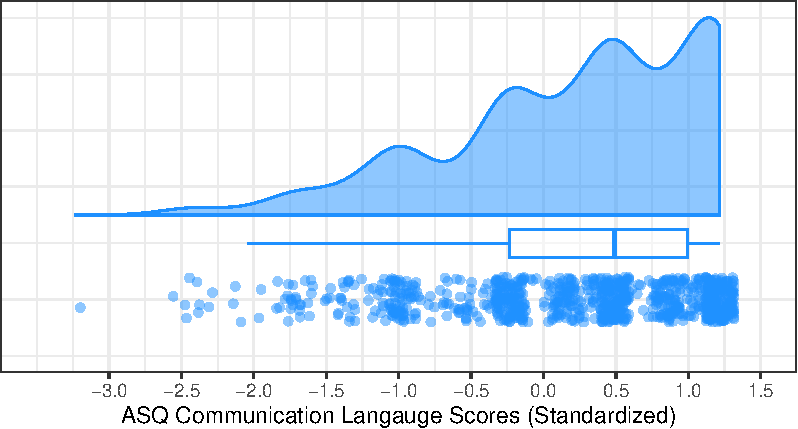
\includegraphics{HWC_progress-report-4_files/figure-latex/fig_rain_ASQ-1} 

}

\caption{Distribution of ASQ communication language scores}\label{fig:fig_rain_ASQ}
\end{figure}

\subsection{Bivariate Analyses}\label{bivariate-analyses}

\begin{figure}[H]

{\centering 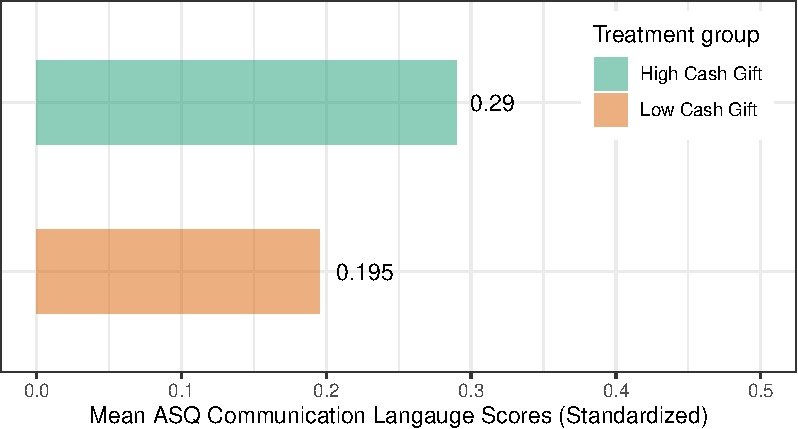
\includegraphics{HWC_progress-report-4_files/figure-latex/fig_bar_treat_ASQ-1} 

}

\caption{Mean ASQ communication language scores by Treatment Group}\label{fig:fig_bar_treat_ASQ}
\end{figure}

\begin{figure}[H]

{\centering 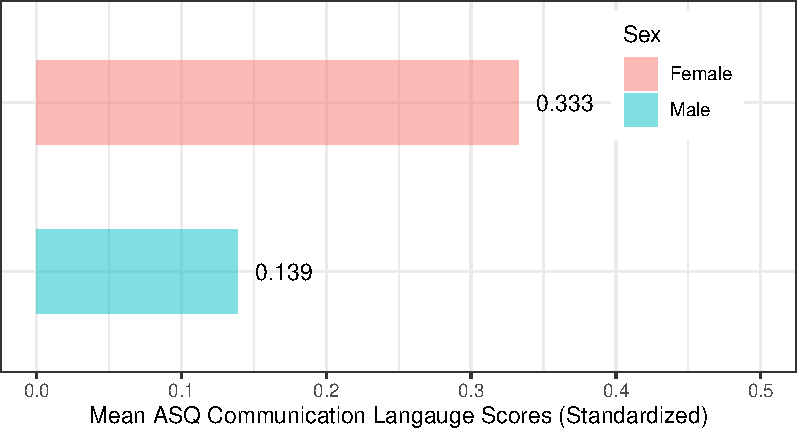
\includegraphics{HWC_progress-report-4_files/figure-latex/fig_bar_sex_ASQ-1} 

}

\caption{Mean ASQ communication language scores by Sex}\label{fig:fig_bar_sex_ASQ}
\end{figure}

\begin{figure}[H]

{\centering 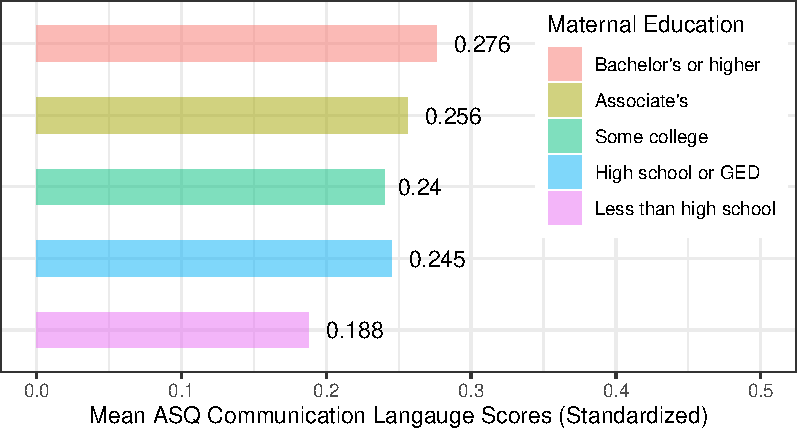
\includegraphics{HWC_progress-report-4_files/figure-latex/fig_bar_medu_ASQ-1} 

}

\caption{Mean ASQ communication language scores by Maternal Education}\label{fig:fig_bar_medu_ASQ}
\end{figure}

\section{Model Development}\label{model-development}

\subsection{Model Selection}\label{model-selection}

\begin{itemize}
\tightlist
\item
  Elastic net was chosen because of number of cases was low
  (\textless2,000).
\item
  Random forest was also chosen because high number of features
  (\textasciitilde170)
\end{itemize}

\subsection{Hyperparameter Tuning}\label{hyperparameter-tuning}

\begin{itemize}
\tightlist
\item
  Elastic net

  \begin{itemize}
  \tightlist
  \item
    Monte Carlo resamples
  \item
    Regular grid research with 500 levels for both mixture and penalty
  \item
    Evaluation metric was RMSE
  \end{itemize}
\item
  Random Forest

  \begin{itemize}
  \tightlist
  \item
    Monte Carlo resamples
  \item
    1000 trees
  \item
    Regular grid research with 50 levels for mtry (between 10 to 100)
    and min\_n
  \item
    Evaluation metric was RMSE
  \end{itemize}
\end{itemize}

\section{Model Performance}\label{model-performance}

\begin{itemize}
\tightlist
\item
  RMSE was used as the performance metric
\end{itemize}

\subsection{Evaluation on Testing Set}\label{evaluation-on-testing-set}

Elastic net final model performance on testing set:

\begin{verbatim}
## # A tibble: 2 x 4
##   .metric .estimator .estimate .config             
##   <chr>   <chr>          <dbl> <chr>               
## 1 rmse    standard     0.841   Preprocessor1_Model1
## 2 rsq     standard     0.00237 Preprocessor1_Model1
\end{verbatim}

\subsection{(Optional) Comparison Across
Models}\label{optional-comparison-across-models}

\begin{itemize}
\tightlist
\item
  Compare the elastic net model results with a random forest model.
\end{itemize}

\section{Discussion}\label{discussion}

\subsection{Implications and Use Cases
Revisited}\label{implications-and-use-cases-revisited}

\subsection{Limitations and Future
Work}\label{limitations-and-future-work}

\section{Appendix}\label{appendix}

~

\bibliography{bibliography.bib}


\end{document}
